\documentclass[10pt,twocolumn,twoside]{genpaper}
\usepackage[numbers,sort&compress]{natbib}

\newcommand{\npscarf}{$\mathtt{npScarf}$}
\newcommand{\npscarfg}{$\mathtt{npScarf\_wag}$}
\newcommand{\npreader}{$\mathtt{npReader}$}
\newcommand{\npanalysis}{$\mathtt{npAnalysis}$}
\newcommand{\npbarcode}{$\mathtt{npBarcode}$}
\newcommand{\npgraph}{$\mathtt{npGraph}$}
\newcommand{\canu}{$\mathtt{Canu}$}
\newcommand{\unicycler}{$\mathtt{Unicycler}$}
\newcommand{\spades}{$\mathtt{SPAdes}$}
\newcommand{\albacore}{$\mathtt{Albacore}$}
\newcommand{\racon}{$\mathtt{Racon}$}
\newcommand{\metrichor}{$\mathtt{Metrichor}$}
\newcommand{\minimap}{$\mathtt{minimap2}$}
\newcommand{\miniasm}{$\mathtt{miniasm}$}
\newcommand{\bwa}{$\mathtt{BWA\text{-}MEM}$}

\newcommand{\ec}{\emph{E.~coli}}
\newcommand{\sce}{\emph{S.~cerevisae}}
\newcommand{\kp}{\emph{K.~pneumoniae}} 

\newcommand{\IE}{\emph{i.e.}}
\newcommand{\EG}{\emph{e.g.}}
\newcommand{\review}[1]{\textcolor{red}{#1}}

\newcommand{\cthead}[2]{\multicolumn{#1}{c}{\textbf{#2}}}
\definecolor{Gray}{gray}{0.9}
\newcommand{\cir}{$^\ast$}
\newcommand{\bres}[1]{{\bf #1}}

\usepackage{pdfpages} 
\usepackage{mathtools}
\usepackage{play}
\usepackage{makeidx}
\usepackage{xcolor,colortbl}
\usepackage{longtable}
\usepackage{booktabs}
\usepackage{hyperref}
\usepackage{pdflscape}

\usepackage{amsmath,amsfonts,amssymb} % this is handy for mathematicians and physicists
			      % see http://www.ams.org/tex/amslatex.html

% \usepackage{showkeys} % this shows what labels you are using for cross
		      % references

\usepackage{graphicx} % standard graphics package for inclusion of
		      % images and eps files into LaTeX document

\usepackage{multirow} 

% For pseudocode
\usepackage[linesnumbered,boxed,ruled,vlined]{algorithm2e}
\newcommand\mycommfont[1]{\footnotesize\ttfamily\textcolor{blue}{#1}}
\SetCommentSty{mycommfont}
% For code embedding (Bash, Java...)
\usepackage{listings}
\lstset{basicstyle=\ttfamily,
  showstringspaces=false,
  commentstyle=\color{red},
  keywordstyle=\color{blue}
}

\usepackage{float}
\usepackage[caption = false]{subfig}
% this code hacked from that of R Chandrasekhar from UWA
\newif\ifpdf
\ifx\pdfoutput\undefined
	\pdffalse    % we are not running pdfLaTeX
\else
	\pdfoutput=1 % we are running pdfLaTeX
	\pdftrue
\fi

\ifpdf
	\DeclareGraphicsExtensions{.pdf}  % this command defined in graphicx
	\pdfcompresslevel=9  % 0: no compression, 9: highest compression
			     % or, set compress_level 9 in file pdftex.cfg
\else
	\DeclareGraphicsExtensions{.ps}
\fi

\usepackage{xr}
\externaldocument{supplementary}
%%%%%%%%%%%%%%%%%%%%%%%%%%%%%%%%%%%%%%%%%%%%%%%%%%%%%%%%%%%%%%%%%%%%%%%%%%%%%%
%%%%%%%%%%%%%%%%%%%%%%%%%%%%%%%%%%%%%%%%%%%%%%%%%%%%%%%%%%%%%%%%%%%%%%%%%%%%%%
%% Some functions provided  by the class

%Display line numbers on the margins
\lineno

%Display watermark DRAFT
%\watermark{DRAFT}

%% use \onecolumn for onecolumn paper
\onecolumn

%Set the title
\title{Online resolving assembly graph by long reads data}

%Set the short tittle
\shorttitle{An awesome paper}

%Authors
\author[1,$\dag$, $\ast$]{Author First}
\author[1,$\dag$]{Author Two} 
\author[1,2]{Author Three}
\author[1,2,$\ast$]{Author Last}

%Affiliation
\affil[1]{Affiliation One}
\affil[2]{Affiliation Two}

%Display equal author textrent focus is developing methods to determine evolutionary relationships, primarily usi
\equalauthors{\textsuperscript{$\dag$}These authors contributed equally to
this work.}

%Display correspondingauthor text 
\correspondingauthor{
\textsuperscript{$\ast$}To whom correspondence should be addressed. E-mails:
author.last\@email.com,author.first\@email.com}

%Display ``This manuscript was compiled on XXXX''
\compiledate

%Set abstract (see below)
\abstract{This is abstract}

%Set keywords
\keywords{Keyword 1, Keyword 2,Keyword 3}

%%%%%%%%%%%%%%%%%%%%%%%%%%%%%%%%%%%%%%%%%%%%%%%%%%%%%%%%%%%%%%%%%%%%%%%%%%%%%%

\begin{document}
%Abstract and keywords have to be defined before \maketitle
\maketitle
\thispagestyle{fancy}

%%%%%%%%%%%%%%%%%%%%%%%%%%%%%%%%%%%%%%%%%%%%%%%%%%%%%%%%%%%%%%%%%%%%%%%%%%%%%%%%%%%
\section{Introduction}
% \begin{itemize}
% \item The importance of having a real-time assembler for bacterial and small genomes: e.g. npscarf 
% \item The difficulty to resolve assembly graph in real-time.
% \item Available hybrid assembly methods using long reads: unicycler, ...
% \item an online algorithm to resolve assembly graph by long reads is needed, ...
% \item Requirements
%     \begin{itemize}
%     \item Support streaming: efficient with high yield (armortized analysis)
%     \item Statistically robust: online modification of the dynamic graph, back tracking edge deletion...
%     \item Standardisation : output GFA in real-time
%     \end{itemize}
% \end{itemize}
Streaming assembly methods have been proven to be useful in saving time and resources compared to the traditional batch algorithms with examples included \EG $\mathtt{Faucet}$~\cite{Rozov2017faucet} and \npscarf{}~\cite{Cao2017scaffolding}. The first method allows the assembly graph to be constructed incrementally as long as reads are retrieved and processed. This practice is helpful dealing with huge short-read data set because it can significantly reduce the local storage for the reads, as well as save time for a DBG construction while waiting for the data being retrieved.

\npscarf{}, on the other hand, works on the available short-read assembly to scaffold the contigs using nanopore sequencing which is well-known by the real-time property. The completion of genome assembly along with the sequencing run provides explicit benefits in term of resource control and turn-around time for analysis~\cite{Cao2017scaffolding}.  
However, due to the greedy approach of a streaming algorithm, as well as being an alignment-based-only scaffolding mechanism, running the tool with default settings suffers from mis-assemblies~\cite{Wick2017unicycler,Giordano2017}. In many case, the gap filling step has to rely on the low quality nanopore reads thus the accuracy of the final assembly is affected as well. 
To tackle the quality issue while maintaining its streaming execution, an assembly graph processing system is investigated as it would provide an additional high-quality source of linking information for the assembly operations. 

After the construction of an assembly graph, the next step is to traverse the graph, resolve the repeats and identify the longest possible un-branched paths that would represents contigs for the final assembly.
Hybrid assembler using nanopore data to resolve the graph has been implemented in $\mathtt{hybridSPAdes}$ \cite{AntipovKM2015} or \unicycler{} \cite{Wick2017unicycler}. 
In general, the available tools employ batch-mode algorithms on the whole long-read data set to generate the final genome assembly. 
In which, the \spades{} hybrid assembly module, from its first step, exhaustively looks for the most likely paths (with mininum edit distance) on the graph for each of the long read given but only ones supported by at least two reads are attained. In the next step, these paths will be subjected to a decision-rule algorithm, namely $\mathtt{exSPAnder}$~\cite{Prjibelski2014}, for repeat resolution by step-by-step expansion, before output the final assembly.
On the other hand, \unicycler{}'s hybrid assembler will initially generate a consensus long read for each of the bridge from the batch data. 
The higher quality consensus reads are used to align with the assembly graph to find the best paths bridging pairs of anchored contigs.
While the later approach employs the completeness of the data  set from the very beginning for a consensus step, the former only iterates over the batch of possible paths and relies on a scoring system for the final decision of graph traversal. For that reason, the first direction is more suitable for a real-time pipeline.
    
However, the challenges to adapt this approach into a real-time mechanism are obvious and mainly come from the heavy path-finding task and the complication of self-improvement step which is critical to a streaming algorithm. 
A modified DFS algorithm and a voting system with accumulating scores calculation has been implemented to overcome these issues.
This results in \npgraph{}, an user-friendly tool with GUI that can traverse the assembly graph and scaffold its components in real-time as long as the nanopore sequencing process is running and continuously generating long reads.  
%%%%%%%%%%%%%%%%%%%%%%%%%%%%%%%%%%%%%%%%%%%%%%%%%%%%%%%%%%%%%%%%%%%%%%%%%%%%%%%%%%%
\section{Results}
\subsection{\npgraph{} -- a tool to resolve assembly graph in real-time}
\npgraph{}'s input consists of Illumina assembly graph resulted from running assembler, e.g. \spades{}~\cite{BankevichNA2012}, $\mathtt{Velvet}$ \cite{Zerbino2008}, $\mathtt{AbySS}$ \cite{Simpson2009} on Illumina short reads, together with long reads from third generation sequencing technology (Oxford Nanopore Technology, Pacbio).
The long reads will be aligned with the contigs in the assembly graph to indicate longer paths that should be traversed. These local paths, given sufficient data, are expected to untangle the complicated graph and guide to the global Eulerian paths (or cycles if possible) that represent the entire genomic sequences. 
\npgraph{} can be invoked and fully function from the command-line interface. In addition, in order to aid the visualization of the assembly process, a GUI has been developed as well.

\begin{figure}[!hpt]
\centering
\parbox{\textwidth}{
    \parbox{.57\textwidth}{
        \subfloat{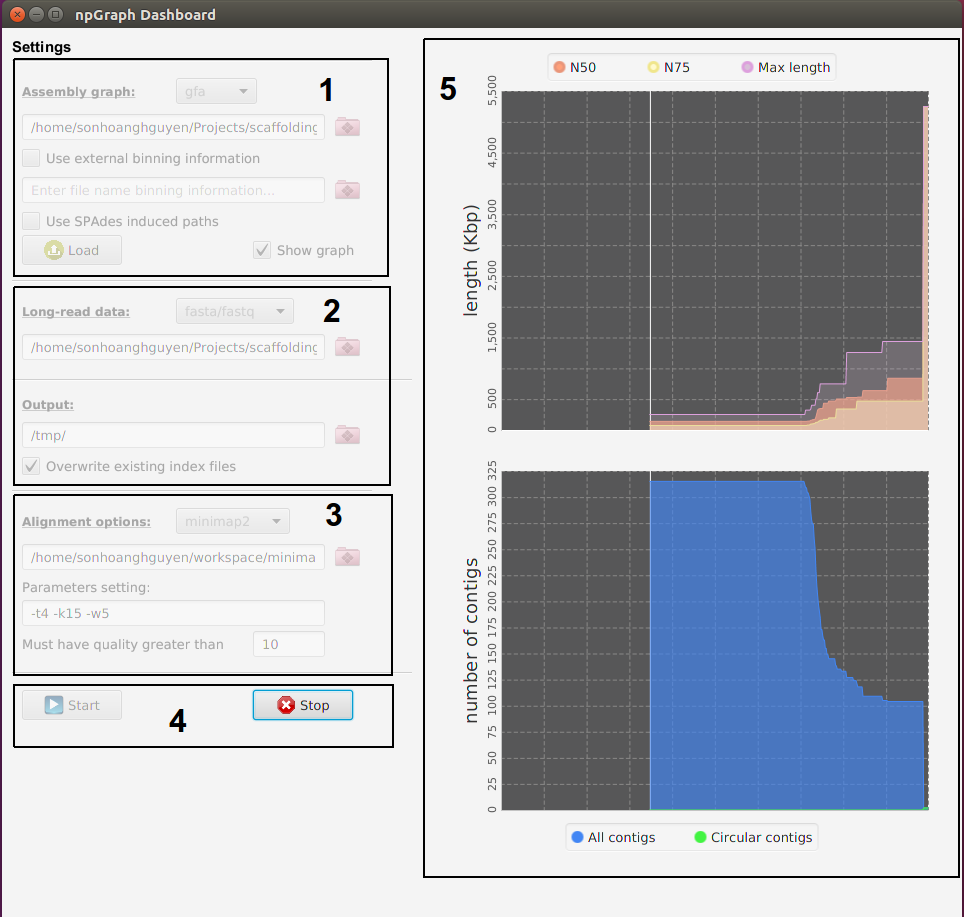
\includegraphics[width=\hsize]{images/dashboard.png}}
    }
    \hskip1em
    \parbox{.44\textwidth}{%
        \subfloat{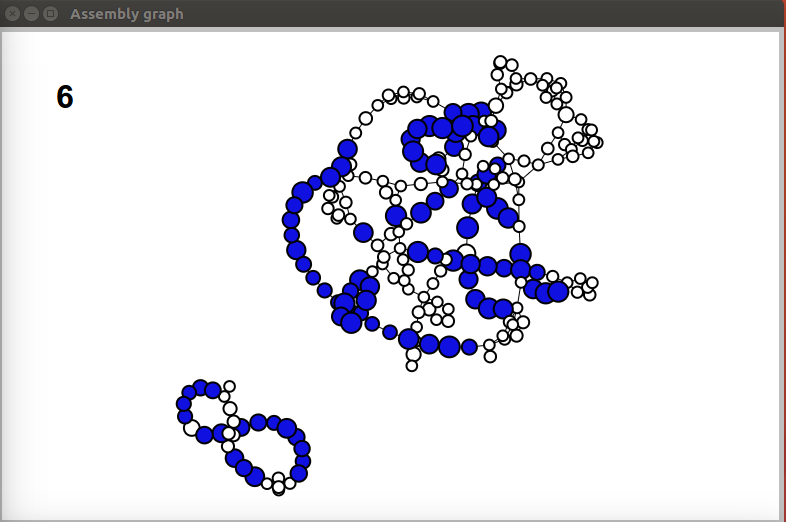
\includegraphics[width=\hsize]{images/graph-view.png}}
        \vskip1em
        \subfloat{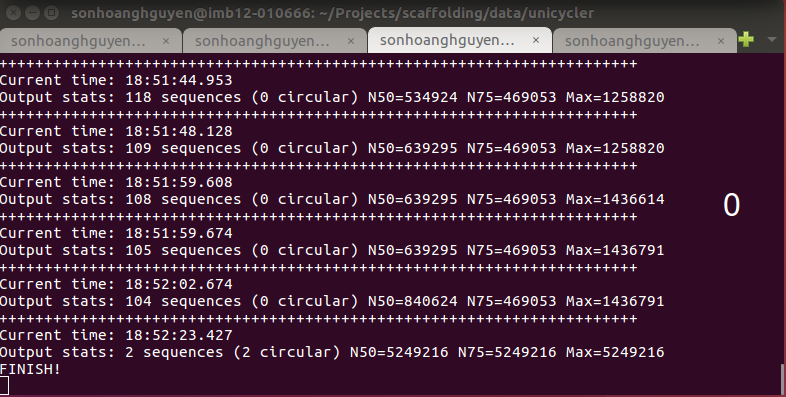
\includegraphics[width=\hsize]{images/console-view.png}}  
    }
}
\caption[\npgraph{} user interface]{\npgraph{} user interface including Console (\textbf{0}) and GUI components (\textbf{1}-\textbf{6}). The GUI consists of the Dashboard (\textbf{1}-\textbf{5}) and the Graph View (\textbf{6}). From the Dashboard there are 5 components as follow: \textbf{1} the assembly graph input field; \textbf{2} the long reads input field; \textbf{3} the aligner settings field; \textbf{4} control buttons (start/stop) to monitor the real-time scaffolding process; \textbf{5} the statistics plots for the assembly result.}
\label{figure:npgraph_gui}
\end{figure}

The GUI includes the dashboard for control the settings of the program and another pop-up window for a simple visualization of the assembly graph in real-time (Figure~\ref{figure:npgraph_gui}).
In this interface, the assembly graph loading stage is separated from the actual assembly process so that users can check for the graph quality first before carry out any further tasks. The box numbered \textbf{1} on Figure~\ref{figure:npgraph_gui} is designed for this task.
Only after an assembly graph is loaded successfully, users can move to box \textbf{2} to specify the nanopore input data.
Settings for an aligner (\bwa{} or \minimap{}) in box \textbf{3} is required if the input is the raw sequences in FASTA/FASTQ format. Another option is to run the alignment independently and provide SAM/BAM input for the next stage of bridging and assembly. This stage is controlled by buttons in box \textbf{4}: the START button ignites the process while the STOP button can prematurely terminate it and output the assembly result till that moment. The plots from the right panel (\textbf{5}) depicts real-time statistics of the assembly contigs inferred from the graph.
From the second window (\textbf{6}), the colored vertices imply unique contigs while the white ones involve either unspecified or repetitive elements. The number of different colors (other than white) indicates the amount of abundant groups being detected as population bins (\EG{} chromosome versus different plasmids, or different bins in metagenomics).

A proper combination of command line and GUI can provide an useful streaming pipeline that copes well with MinION output data. The practice is similar to the previous developed pipelines~\cite{CaoGC2016,Cao2017scaffolding,Nguyen2017barcode} that allow the analysis to take place abreast to a nanopore sequencing run.

\subsection{Hybrid assembly for synthetic data sets}
To evaluate the performance of the method, \npgraph{} was benchmarked against \spades{} with its hybrid assembly module~\cite{AntipovKM2015}, \npscarf{} with/without assembly graph integrated, and Unicycler version 0.4.6 on the latter's testing data~ \cite{Wick2017unicycler} . This data set were simulations of Illumina and MinION raw data, generated \emph{in silico} based on random and available microbial references. 
Specifically, the synthetic Illumina data was generated by using a wrapper script of ART~\cite{HuangLMM2012} that allows uniform coverage for circular genome sequencing with justifiable depths.
PBSIM~\cite{OnoAH2012}, on the other hand, was used to simulate the long reads.

There were three settings for each of the synthetic raw data (\emph{good, medium, bad}) corresponding to the quality, yield and length of reads being generated. 
In the SGS simulation, the \emph{bad} data consist of 100bp paired-end reads with low and uneven coverage (40X) leading to many dead ends in the assembly graph due to missing regions in the genome. 
The read length was 125bp in the \emph{medium} setting with better depth distributions that could cover the genome better. 
Finally, the \emph{good} option provided best data sets with 150bp of read length and 100X coverage.
While the quality of SGS reads would determine the assembly graph nature, the nanopore data plays critical role in graph resolving.
The three settings leveled up the depth (8X, 16X, 32X) and at the same time, average length ($5$Kbp, $10$Kbp, $20$Kbp) and maximum identities (90\% ,95\% ,98\%) respectively.
We only considered the \emph{good} configurations of both platforms for the sequence data being tested.
Also, since the other comparative tools do not support streaming assembly, there were only batch-mode runs being carried out and the reciprocal results were examined by QUAST 5.0.2~\cite{Mikheenko2018quast5}. 

\LTcapwidth=\linewidth
% \footnotesize
\begin{longtable}{llcrrrrr@{\hspace{2pt}}c@{\hspace{2pt}}r}
\caption[Comparison of assemblies using \npgraph{} and other comparative methods on 5 synthetic data sets]{Comparison of assemblies produced in batch-mode using \npgraph{} and the comparative methods on 5 synthetic data sets taken from \url{https://cloudstor.aarnet.edu.au/plus/index.php/s/dzRCaxLjpGpfKYW}} \label{table:npgraph_compare} \\

 \toprule
    &       & \cthead{1}{Assembly} &     & 
    \cthead{1}{N50}  & \cthead{1}{Mis-} &  \cthead{1}{Error}  &
    \cthead{3}{Run times} \\
    & \cthead{1}{Method} & \cthead{1}{size (Mb)} & \cthead{1}{\#Contigs} &
    \cthead{1}{(Kp)} & \cthead{1}{assemblies} & \cthead{1}{(per 100 Kb)} &  
    \cthead{3}{(CPU hrs)} \\
\toprule    
\endfirsthead

\multicolumn{10}{c}%
{{\tablename\ \thetable{} -- continued from previous page}} \\
 \toprule
    &       & \cthead{1}{Assembly} &     & 
    \cthead{1}{N50}  & \cthead{1}{Mis-} &  \cthead{1}{Error}  &
    \cthead{3}{Run times} \\
    & \cthead{1}{Method} & \cthead{1}{size (Mb)} & \cthead{1}{\#Contigs} &
    \cthead{1}{(Kp)} & \cthead{1}{assemblies} & \cthead{1}{(per 100 Kb)} &  
    \cthead{3}{(CPU hrs)} \\
\toprule    
\endhead

\hline \multicolumn{10}{|r|}{{Continued on next page}} \\ \hline
\endfoot

\hline \hline
\endlastfoot

\rowcolor{Gray} \multicolumn{10}{l}
{ random sequence with repeats} \\*  
 & SPAdes  & 3.928 & 226  & 40.5  &  0 &  0.00 &  0.95 &  &  \\*
 & SPAdes-Hybrid  & 4.109 & 3  & 4,000.0  & 0  & 0.85  & 1.196  &  &  \\*
 & Unicycler  & 4.110 & 3  & 4,000.0  &  0 &  0.47 & 6.783  &  &  \\*
 & npScarf  & 4.251 &  9 & 3,952.2  &  27 &  8.74 &  0.95 & + & 0.39 \\*
 & npScarf\_wag & 4.554 & 9  &  3,999.6 &  37 &  6.16 &  0.95 & + &  0.45\\*
 & npGraph (bwa)  & 4.110 & 3  & 4,000.0  & 0  &  0.47 &  0.95 & + &  0.33\\*
 & ngGraph (minimap2)  & 4.110 & 3  & 4,000.0  & 0  & 0.47  &  0.95 & + &  0.02\\
\rowcolor{Gray} \multicolumn{10}{l}
{\emph{Mycobacterium tuberculosis} H37Rv} \\*  
 & SPAdes  & 4.371 & 114  &  125.5 &  1 & 1.51  &  1.55 &  &  \\*
 & SPAdes-Hybrid  & 4.411 & 1  & 4,411.2  & 0  & 1.73  & 1.68  &  &  \\*
 & Unicycler  & 4.412 &  1 &  4,411.5 & 0  &  2.56 &  6.36 &  &  \\*
 & npScarf  & 4.446 & 4  & 4,389.9  & 12  &  11.41 & 1.55  & + & 0.78 \\*
 & npScarf\_wag  & 4.408 & 1  & 4,407.6  &  2 &  7.01 & 1.55  & + & 0.79 \\*
 & npGraph (bwa)  & 4.411 &  1 & 4,411.6  &  0 & 7.28  &  1.55 & + & 0.63 \\*
 & ngGraph (minimap2)  & 4.411 & 1 & 4,411.4  &  0 &  7.01 & 1.55  & + &  0.02\\
\rowcolor{Gray} \multicolumn{10}{l}
{\ec{} O25b H4-ST131} \\*  
 & SPAdes  & 5.173 &  159 & 191.0  &  1 &  1.69 & 1.26  &  &  \\*
 & SPAdes-Hybrid  & 5.249 &  7 &  5,109.6 & 0  & 2.65  & 1.40  &  &  \\*
 & Unicycler  & 5.249 &  3 & 5,109.8  &  0 &  4.29 &  4.70 &  &  \\*
 & npScarf  & 5.354 & 7  & 5,087.5  &  14 & 29.12  &  1.26 & + &  0.78\\*
 & npScarf\_wag  & 5.413 &  7 & 5,108.1  & 6  &  30.29 & 1.26  & + & 0.78 \\*
 & npGraph (bwa)  & 5.252 & 3  &  5,112.3 &  0 & 16.37  & 1.26  & + &  0.66\\*
 & ngGraph (minimap2)  & 5.250 & 3  & 5,111.1  & 0  & 14.61  &  1.26 & + & 0.03 \\
\rowcolor{Gray} \multicolumn{10}{l}
{\emph{Streptococcus suis} BM407} \\*  
 & SPAdes  & 2.119 &  81 &  131.0 & 0  & 3.84  & 0.59  &  &  \\*
 & SPAdes-Hybrid  & 2.147 & 48  &  1,438.0 &  0 &  0.98 & 0.65  &  &  \\*
 & Unicycler  & 2.171 &  2 &  2,146.2 & 0  &  2.99 &  2.58  &  &  \\*
 & npScarf  & 2.220 &  4 &  2,120.0  & 9  & 97.20  & 0.59 & + & 0.31 \\*
 & npScarf\_wag  & 2.245 & 4  &  2,128.3  & 3  &  89.64 & 0.59 & + &  0.31\\*
 & npGraph (bwa)  & 2.167 & 6  & 2,146.7  &  0 &  26.77 & 0.59  & + &  0.21\\*
 & ngGraph (minimap2)  & 2.167 & 6  &  2,146.2 &  0 & 22.53  &  0.59 & + & 0.01 \\
\rowcolor{Gray} \multicolumn{10}{l}
{\emph{Acinetobacter} AB30} \\*  
 & SPAdes  & 4.134 & 265  & 42.5  &  0 &  3.23 & 0.95  &  &  \\*
 & SPAdes-Hybrid  & 4.287 & 49  &  3,308.0 &  0 & 5.04  & 1.84  &  &  \\*
 & Unicycler  & 4.333 & 1  &  4,333.0 &  1 & 6.95  &  5.27 &  &  \\*
 & npScarf  & 4.595 & 11  & 4,299.7  & 1  & 120.99  & 0.95  & + & 0.45 \\*
 & npScarf\_wag  & - & -  &  - & -  &  - &  - &  &  \\*
 & npGraph (bwa)  & 4.317 & 6  &  2,766.9 & 1  &  39.82 &  0.95 & + & 0.41 \\*
 & ngGraph (minimap2)  & 4.337 & 1  &  4,336.8 & 0  & 24.71  & 0.95  & + & 0.03 \\
\end{longtable}

\normalsize

Table~\ref{table:npgraph_compare} shows evaluation results for 5 synthetic data sets, the output of the full run can be found in Supplementary Table~\ref{supp_tab:synthetic_benchmark}.
In the first column of applied methods, beside \unicycler{} and $\mathtt{hybridSPAdes}$, the original scaffolder \npscarf{} was included as well as \npscarfg{} -- its modified version with assembly graph integrated.
On the other hand, \npgraph{} can use 2 different aligners, \bwa{} and \minimap{}, for its bridging phase thus both practices were included in this comparison.

In general, the graph integrated version of \npscarf{} improved the assembly results in terms of mis-assemblies and error reduction while virtually consuming similar resources compared to the original version.
The only exception where the number of mis-assemblies being increased was the simulation of a random sequence with many repeats. There were 10 more mistakes detected using the later version \npscarfg{}. However, with additional investigations, we found that the number of mis-assemblies on the true positive circular sequences (3 from the reference) has been significant reduced by applying assembly graph for \npscarf{}. The errors mostly came from redundant sequences output from the software due to the failure in estimation of contig multiplicity.
Even though using assembly graph for gap fillings, there were no changes in the way to determine if a contig is unique or not from \npscarfg{}. 
It still relied on the length and coverage statistics, \IE{} \emph{Astats}~\cite{MyersSD2000} to find anchors that were critical for the backbone construction of the assembly.
Redundant path findings for false positive replicons consequently returned additional wrong translocations in the final contigs which were reported by QUAST. 
Other than that, the method had successfully produced better assemblies than the original. Regarding \emph{Mycobacterium tuberculosis} H37Rv, the number of mis-assembled breakpoints had been trimmed down from 12 to 2, while the number of final contigs had reduced from 4 to only one as in the reference. Results in cases of \ec{} O25b H4ST131 and \emph{Streptococcus suis} BM407 also showed enhancements in terms of those categories as well as N50 statistics. 
There was improvements considering the nucleotide errors (mismatches and indels) as well from aforementioned data sets, except for the \ec{} when slightly more mismatches had been detected. However, these errors can be corrected by running polishing tools with the raw Illumina data afterward. 

For \emph{Acinetobacter} AB30 synthetic data, it was an deficiency for \npscarfg{} in traversing the graph to find candidate paths for a bridge of long distance due to particular large search space.
The exhaustive, naive DFS implementation for this version of \npscarf{} required a lot of memory to traverse a complex assembly graph that usually exceed a normal desktop's capacity.
This issue has been fixed in \npgraph{} when Algorithm~\ref{algo:findpath} was used on the definitive graph. This resulted in completed runs of the assembly process for all data sets with the similar number of mis-assemblies compared to the best figures in this category.
As shown in Table~\ref{table:npgraph_compare} and \ref{supp_tab:synthetic_benchmark}, the assembly graph based methods offered significant improvements when compared to \npscarf{}. Not only because of the clear drops with respect to mis-assemblies and errors, but it was also reflected by the number of final contigs and their N50 as well.

To align the long reads to the assembly graph components, either \bwa{}~\cite{Li2013} or \minimap{}~\cite{Li2016} was invoked in \npgraph{}. 
The former option was inherited from \npscarf{} pipeline with the intact parameters
%$-k11 -W20 -r10 -A1 -B1 -O1 -E1 -L0 -a -Y$
while the latter was used with the recommended settings (-$\mathtt{k}$15 -$\mathtt{w}$5) for the best sensitivity working on MinION data.
Even though, \bwa{} normally reported more hits than \minimap{} but at the same time, was responsible for more false positive alignments.
For instance, regarding the last data set from Table~\ref{table:npgraph_compare}, the assembly of \npgraph{} using \bwa{} was suffered from the ambiguous alignments thus more fragmented than the other counterparts. 
On the other hand, referring to more complicated graphs from \emph{Acinetobacter} A1 and the yeast \emph{Saccharomyces cerevisiae} S288c from Table~\ref{supp_tab:synthetic_benchmark}, the number of mis-assemblies from using \minimap{} were increased due to the lacks of appropriate alignments to support accurate bridging process.
However, under almost circumstances, using either aligners would result in final assemblies with similar qualities.
Furthermore, in terms of running time and resources required, \minimap{} proved to be the best option. 
The total CPU hours had been trimmed down drastically with the new aligner, making \npgraph{} the fastest hybrid assembler available.
This feature is certainly more favoured to a real-time assembly as well.
As the consequence, as long as \minimap{} is expected to replace \bwa{} for long-read sequencing data alignment, it would likewise become the main aligner for \npgraph{} pipeline in the future.

It is noteworthy to discuss in more details the errors addressed in the above assembly methods.
This figure measured the total mismatches and indels per 100kpb from the assembly sequences when mapping to the reference.
As expected from hybrid assemblies where Illumina sequencing data were used as the main building blocks, the figures were hardly bigger than 100 (equivalent to 0.1\% error rate) for almost every case.
In addition, the indels errors, which mainly caused by TGS data, were found relatively low in the final contigs (Table~\ref{supp_tab:synthetic_benchmark}).
The majority of the differences accounted for the mismatched nucleotides caused by the alternative paths connecting the unique anchors from the backbone of the assembly.
This phenomenon may root from homologous repeats or sequencing errors of the genome.
From all the hybrid assemblers, $\mathtt{hybridSPAdes}$ reported results with highest fidelity. This meant that the performance its decision-rule algorithm $\mathtt{exSPAnder}$~\cite{Prjibelski2014} was the most accurate amongst all path finding methods. As the trade-off, there were fewer connections satisfying its quality threshold, resulting in the fragmented assemblies in cases of \emph{Streptococcus suis} or \emph{Acinetobacter} samples (Table~\ref{table:npgraph_compare} and \ref{supp_tab:synthetic_benchmark}).
\unicycler{}, which employs an algorithm based on semi-global (or glocal) alignments~\cite{Brudno2003glocal} with the consensus long reads, returned the second best reliable and at the same time, closest-to-complete results overall.
\npscarf{}, on the other hand, exploited the long reads for the gap filling thus inherited the high error rates from them.
By integrating the assembly graph for the task, the errors were reduced in general (random sequences, \emph{M.~tuberculosis}, \emph{S.suis} from Table~\ref{table:npgraph_compare}) but not completely since the mis-placed contigs were still not resolved in other circumstances.
\npgraph{} significantly reduced the errors compared to \npscarf{}, however the figures were still higher than the those of the best counterparts.
This implied a more robust decision making system is needed in \npgraph{}'s real-time path finding module for even better output's accuracy.

\subsection{Hybrid assembly for real data sets}
Several sequencing data sets of actual bacterial samples~\cite{George2017M14} were used in this scenario.
The data included both Illumina paired-end and MinION sequencing based-call data for each sample.
Unlike previous settings, rather than the default output, the optimal \spades{} assembly graph detected by \unicycler{} were used for \npgraph{} algorithm as well.
This step had been proved to be useful in selecting the best graph available, amongst \spades{} runs with ranging $k$-mer values, that have dead-ends and number of contigs minimized~\cite{Wick2017unicycler}. Likewise, as mentioned before, the quality of the initial assembly graph would considerably influence the final results of \npgraph{}. 

Due to the lack of available reference genomes, fewer statistics were reported by QUAST for the comparison of the results. 
Instead, we investigated the number of circular sequences and $\mathtt{PlasmidFinder}$ 1.3~\cite{Carattoli2014} mappings to obtain an evaluation on the accuracy and completeness of the assemblies.
Table~\ref{tab:npgraph_real} shows the benchmark results of \npgraph{} (using \minimap{}) against \unicycler{} on three data sets of bacterial species \emph{Citrobacter~freundii}, \emph{Enterobacter~cloacae} and \emph{Klebsiella~oxytoca}. 

\begin{table}[!hpt]
\centering
\caption[Assembly of real data sets using \unicycler{} and \npgraph{} with the optimized SPAdes output]{Assembly of real data sets using \unicycler{} and \npgraph{} with the optimized \spades{} output. Circular contigs are highlighted in \textbf{bold}, fragmented assemblies are presented as X$\vert$Y where X is the total length and Y is the number of supposed contigs making up X.}
\label{tab:npgraph_real}
\begin{tabular}{p{4cm}|r|r|l}
 & \unicycler{} & \npgraph{} & Replicons (based on $\mathtt{PlasmidFinder}$ 1.3) \\ \toprule
\emph{Citrobacter freundii} & \textbf{5,029,534} & \textbf{5,029,486} & Chromosome \\
CAV1374 & \textbf{109688} & \textbf{109688} & IncFIB(pHCM2)\_1\_pHCM2\_AL513384 \\
 & \textbf{100,873} & \textbf{100,873} & IncFIB(pB171)\_1\_pB171\_AB024946 \\
 & \textbf{85,575} & \textbf{85,575} & IncL/M(pMU407)\_1\_pMU407\_U27345 \\
 & \textbf{43,621} & \textbf{43,621} & repA\_1\_pKPC-2\_CP013325 \\
 & \textbf{3,223} & \textbf{3,223} & - \\
 & \textbf{1,916} & \textbf{1,916} & ColRNAI\_1\_\_DQ298019 \\
 & 14,464$\vert$3 & 14,456$\vert$2 & - \\ \hline
\emph{Enterobacter cloacae} & 4,806,666$\vert$2 & 4,858,438$\vert$2 & Chromosome \\
CAV1411 & \textbf{90,451} & 90,693$\vert$2 & IncR\_1\_\_DQ449578 \\
 & \textbf{33,610} & \textbf{33,610} & repA\_1\_pKPC-2\_CP013325 \\
 & 13,129$\vert$2 & 14,542$\vert$4 & - \\ \hline
\emph{Klebsiella oxytoca}  & 6,153,947$\vert$5 & \textbf{6,155,762} & Chromosome \\
CAV1015 & \textbf{113,105} & \textbf{113,105} & \begin{tabular}[c]{@{}l@{}}IncFII(SARC14)\_1\_SARC14\_JQ418540;\\ IncFII(S)\_1\_\_CP000858\end{tabular} \\
 & \textbf{111,395} & \textbf{111,395} & - \\
 & \textbf{108,418} & 109,209$\vert$13 & IncFIB(K)\_1\_Kpn3\_JN233704 \\
 & \textbf{76,183} & \textbf{76,186} & IncL/M(pMU407)\_1\_pMU407\_U27345 \\
 & \textbf{11,638} & 11,892$\vert$2 & - \\ \hline
\end{tabular}
\end{table}

From the first data set, there was high similarity between final contigs generated by two assemblers.
They shared the same number of circular ultimate sequences, including the chromosomal and other six replicons contigs. 
The only divergence lied on the biggest sequence ($\simeq 5.029$Mbp) when the \unicycler{}'s chromosome was 48 nucleotides longer than that of \npgraph{}.
Five out of six identical replicons were confirmed as plasmids based on the occurences of appropriate Origin of replication sequences (PlasmidFinder database).
In detail, two megaplasmids (longer than $100$Kpb) were classified as IncFIB while the other two mid-size replicons, $85.6$Kbp and $43.6$Kpb, were incL and repA respectively, leaving the shortest one with $2Kbp$ of length as ColRNAI plasmid.
The remaining circular sequence without any hits to the database was $3.2$Kbp long suggesting that it could be phage or newly replicon's DNA.
Lastly, there were still $14.5$Kbp unfinished sequences resulted in 3 linear contigs from \unicycler{} and 2 for \npgraph{} respectively.

The assembly task for \emph{Enterobacter~cloacae} was more challenging as the chromosomal DNA sequence was not been fully resolved using either method. 
The chromosome size was estimated to be approximately $4.8$Mbp but had been broken into two smaller pieces. 
\npgraph{} returned longer stretches of length $3.324$Mbp and $1.534$Mbp while the figures were $2.829$Mbp and $1.978$Mbp from \unicycler{}'s output.
However, the number of circular sequences detected by \unicycler{} was one more than the other ($2$ versus $1$). They were corresponding to 2 plasmids, namely IncR and repA.
While the latter were recognized by both methods, the longer plasmid sequence was fragmented running \npgraph{}.
Similar to the previous data set, there were around $14$Kpb of data were unable to be finished by the assemblers.

Finally, assembly for \emph{Klebsiella oxytoca} saw fragmented chromosome using \unicycler{} but it was a fully complete contig for \npgraph{} with $6.156$Mbp of size.
The two assemblers shared 3 common circular sequences where two of them were confirmed plasmids. 
The first identical sequences represented a megaplasmid ($\simeq 113$Kbp) with two variations of IncFII's origin of replication DNA being identified. 
The other agreed plasmid were IncL/M with $76$Kbp of length.
Particularly, there was one circular contig with length greater than $100$Kbp but returned no hits to the plasmid database, suggesting the importance of \emph{de novo} replicon assembly in combination with further interrogations.
\unicycler{} detected another megaplasmid of size $108.4$Kbp which was fractured by \npgraph{}. 
The dissolution was also observed in \npgraph{} for the final contig of length $11.6$Kbp where it failed to combine two smaller sequences into one.

In addition to what presented in Table~\ref{tab:npgraph_real}, dot plots for the pair-wise alignments between the assembly contigs were generated and can be found in Appendix Figure~\ref{supp_fig:npgraph_dotplot}. Interestingly, beside all other agreements, there was a structural difference using two methods for \emph{E.~cloacae} CAV1411 genome assembly. This was caused by the inconsistency of a fragment's direction on the final output contigs. However, when compare to a reference genome of the same bacteria strain (GenBank ID: CP011581.1~\cite{Potter2016rapid}), contigs generated by \npgraph{} demonstrated a consistent alignment which was not the case for \unicycler{} results (Appendix Figure~\ref{supp_fig:npgraph_ref}). Even though this might reflect a novel variation between bacterial samples of the same strain, it was more likely a mis-assembly by using \unicycler{}.

Overall, by testing with synthetic and real data, \npgraph{} proved to be able to generate assemblies of comparative quality compared to other powerful batch-mode hybrid assemblers, such as $\mathtt{hybridSPAdes}$ or \unicycler{}.
Furthermore, similar to \npscarf{}, it has the advantage in term of supporting real-time assembly. The next section will address this utility and the interactive GUI bundled in \npgraph{}. 

\subsection{Real-time mode hybrid assembly}
Figure~\ref{F:npgraph_rt} demonstrates the real-time mode performance of \npscarf{} and \npgraph{} via N50 statistics during the assembly of 4 example data sets.
This experiment would discover the rate of completing genome assemblies of the new method, set aside the accuracy aspect which had already been discussed previously.
\npscarf{}\_wg basically scaffolds the pre-assembly contigs in the same manner with the original version thus was not discussed here.

\begin{figure}[!hpt]
\centering
\subfloat[\emph{Citrobacter~freundii} CAV1374]{
	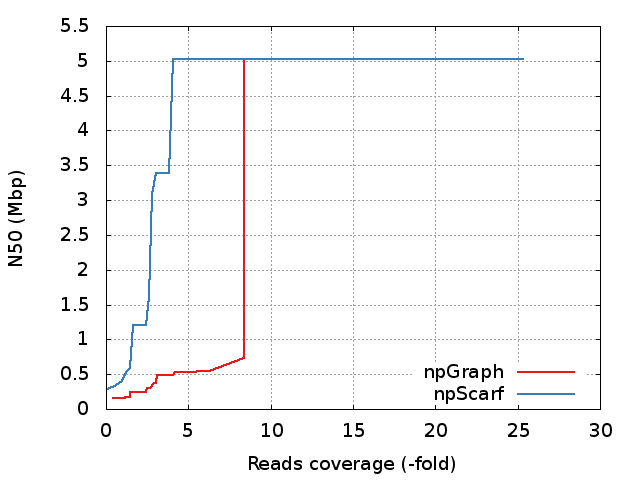
\includegraphics[width=.45\textwidth]{images/rt_cf1374.png}
}
\hfill
\subfloat[\emph{Escherichia~coli} K12 MG1655]{
	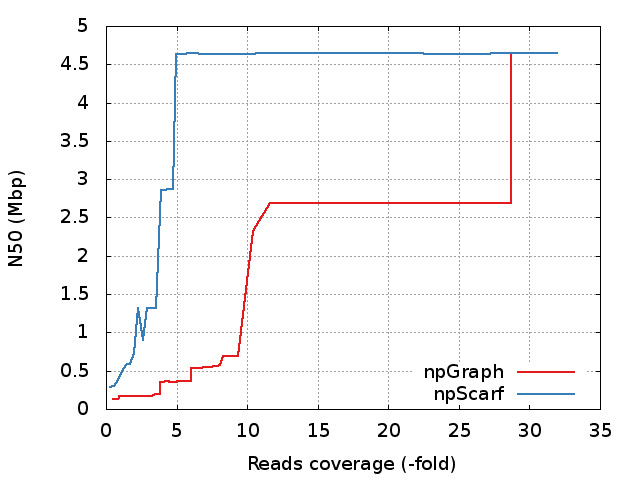
\includegraphics[width=.45\textwidth]{images/rt_eck12.png}
}
\\
\subfloat[\emph{Klebsiella} 30660 NJST258]{
	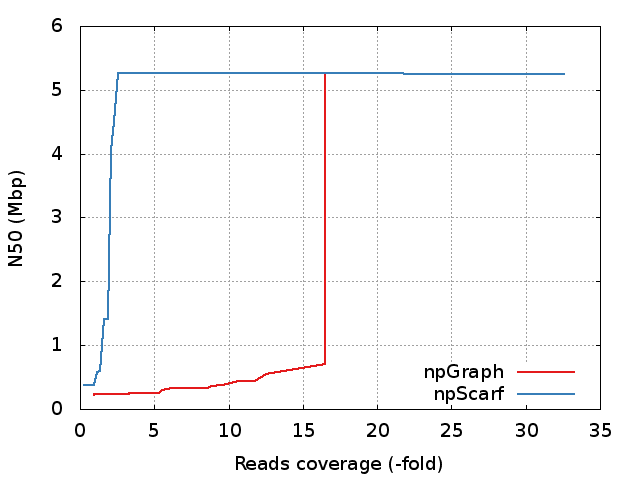
\includegraphics[width=.45\textwidth]{images/rt_kp30660.png}
}
\hfill
\subfloat[\emph{Klebsiella} NTUH K2044]{
	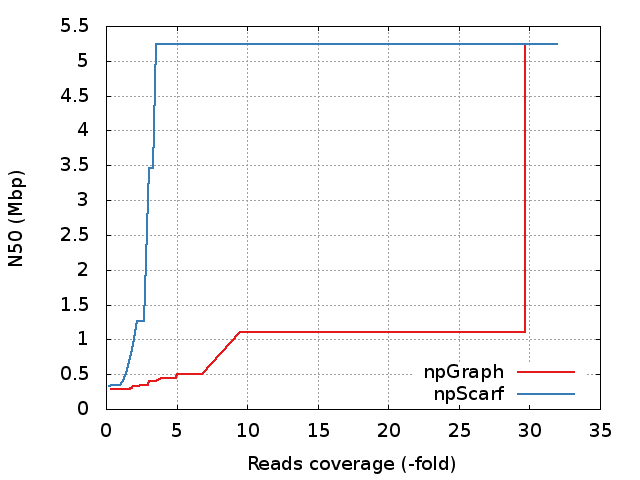
\includegraphics[width=.45\textwidth]{images/rt_kpntuh.png}
}
\caption[Real-time scaffolding by \npscarf{} versus \npgraph{}]{N50 statistics of real-time scaffolding by \npscarf{} versus \npgraph{}.}
\label{F:npgraph_rt}
\end{figure}

As can be observed from all the plots, \npgraph{} and \npscarf{} both converged to the same ultimate completeness but with different paces and patterns.
Apparently it took more data for \npgraph{} to finish the same genome than the other.
The reason stems from the fact that the new algorithm implemented a more `conservative' approach of bridge construction with at least 3 supporting long-reads for each to prevent any potential mis-bridging. 
Unlike \npscarf{} when the connections could be undone and rectified later if needed, a bridge in \npgraph{} will remain unchanged once created.
The plot for \ec{} data clarifies this behaviour when a fluctuation can be observed in \npscarf{} assembly at $\simeq 3$-folds data coverage.
On the other hand, the N50 length of \npgraph{} is always a monotonic increasing function. 
The sharp `jumping' patterns suggested that the linking information from long-read data had been stored and exploited at certain time point decided by the algorithm.
Once a unique path has been determined, the bridge can be formed to connect the fragments together into longer sequences.


\begin{figure}[!hpt]
\centering
\subfloat[Initial graph]{
	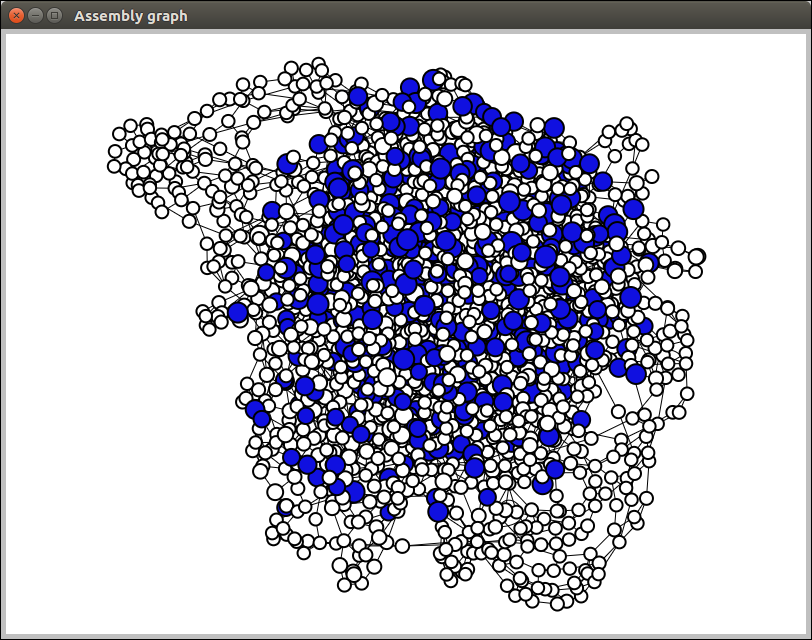
\includegraphics[width=.45\textwidth]{images/npgraph_shigella_0.png}
}
\hfill
\subfloat[Resolved graph]{
	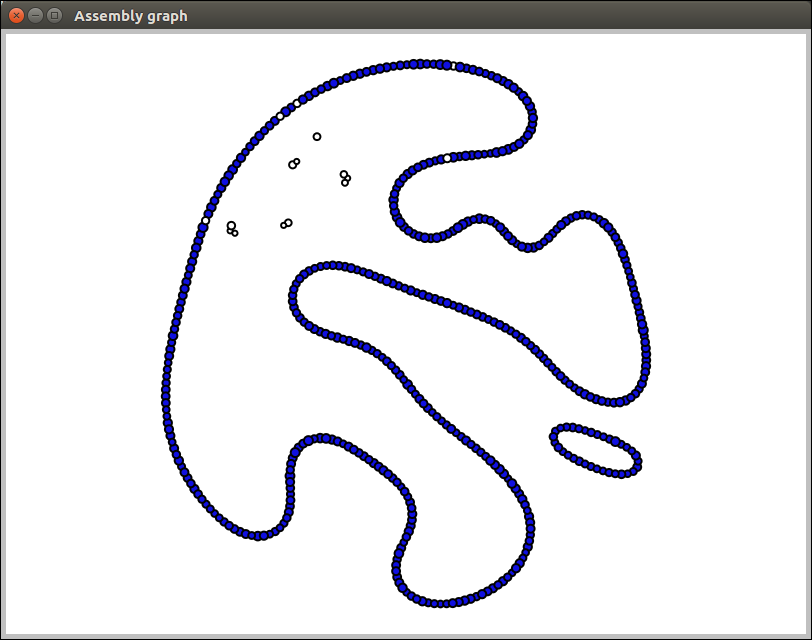
\includegraphics[width=.45\textwidth]{images/npgraph_shigella_2.png}
}
\caption[Assembly graph resolving on \npgraph{} Graph View]{Assembly graph of \emph{Shigella~dysenteriae} Sd197 synthetic data being resolved by \npgraph{} and displayed on the GUI Graph View. The \spades{} assembly graph contains 2186 nodes and 3061 edges, after the assembly shows 2 circular paths representing the chromosome and one plasmid.}
\label{F:npgraph_graphview}
\end{figure}

Figure~\ref{F:npgraph_graphview} shows an example of the real-time graph resolving process being displayed on GUI.
The result graph, after cleaning, would only report the significant connected components that represents the final contigs.
Smaller fragments, even unfinished but with high remaining coverage, are also presented as potential candidates for further downstream analysis.
Further annotation utility can be implemented in the future better monitoring the features of interests as in \npscarf{}.
%%%%%%%%%%%%%%%%%%%%%%%%%%%%%%%%%%%%%%%%%%%%%%%%%%%%%%%%%%%%%%%%%%%%%%%%%%%%%%%%%%%
\section{Conclusions}
Assembly graph is the data structure describing the assembly process at a lower level of more details.
The current chapter brings this informative knowledge to the original \npscarf{}'s mechanism in two ways, either partly for the gap-filling module only (\npscarfg{}) or completely as the building block of the assembly construction method (\npgraph{}).

While the first approach showed improvements in terms of base's accuracy for the final results, it had limited ability in rectifying the mis-assemblies from the original version due to false positive alignments at contig level.
The issue can be tackled by applying the assembly graph completely as in \npgraph{}.
With a more conservative bridging method applied, the new method may consume more data to confidently construct the assembly but at the same time, the number of mis-located fragments has reduced significantly.
Furthermore, users can monitor the assembly in an interactive way providing the assembly GUI.

Compared to the other hybrid assemblers of similar methodology, such as $\mathtt{hybridSPAdes}$ and \unicycler{}, there are still rooms for further development of \npgraph{}. 
More comprehensive pre-processing step is needed for a better input graph possible since it would affect the completeness of final results. 
Importantly, a robust real-time voting system should be implemented to be able to detect the most probable path amongst all candidates in an efficient way.
This would alleviate the data consumption of the \npgraph{} while at the same time, maintain high confident and accurate scaffolding. 


%%%%%%%%%%%%%%%%%%%%%%%%%%%%%%%%%%%%%%%%%%%%%%%%%%%%%%%%%%%%%%%%%%%%%%%%%%%%%%%%%%%
\section{Methods}

Basically the work flow of \npgraph{} can be divided into 3 main phases: abundance binning, graph resolving and assembly output. 
The first step will try to bin the contigs into different groups of \emph{population} based on their coverage. 
Each population would include contigs of the similar abundance in the final assembly sequences, \EG{} chromosome , plasmids, or even particular species genome in a metagenomics community.
The binning phase would assist to differentiate between repetitive contigs and unique ones. By using this information, in combination with path inducing from long reads, the assembly graph is then traversed and resolved in real-time. Finally, the graph is subjected to the last attempt of resolving and cleaning, as well as output the final results. The whole process can be managed by using either command-line interface or GUI.
\subsection{Pre-processing: identify repeat and unique contigs}
The purpose of this step is to investigate the sequencing properties of contigs, \IE{} length and \emph{k-mer} count, in combination with the graph topology, for an initial binning algorithm to determine multiplicity for each of them.
%\paragraph{Correct coverage bias due to GC content}
%The read coverage from Illumina data could be rectified by applying GC-content correction model \cite{BenjaminiS2012}.
%To be implemented.

\paragraph{Initial binning contigs into groups of abundances}
Each contig is represented as a node in the assembly graph and the edge between two nodes indicate their overlap (link) properties.
This step is to cluster the significant nodes (longer than $10$Kbp) into different sets, namely significant abundance groups, based on their coverage values. 

DBSCAN clustering algorithm \cite{Ester96adensity-based} is applied for this task.
The idea is to consider a coverage value of a significant contig (which consists of more than 10,000 \emph{k-mers}) to be a sampled mean of a Poisson distribution (of \emph{k-mers} count). 
The metric is a distance function based on Kullback-Leibner divergence \cite{Kullback1951information}, or relative entropy, of two Poisson distributions.

Assume there are 2 Poisson distribution $P_1$ and $P_2$ with density functions $$p_1(x,\lambda_1)=\frac{e^{-\lambda_1}\lambda_1^x}{\Gamma(x+1)}$$ and $$p_2(x,\lambda_2)=\frac{e^{-\lambda_2}\lambda_2^x}{\Gamma(x+1)}$$ 
The Kullback-Leibner divergence from $P_2$ to $P_1$ is defined as:
$$D_{KL}(P_1||P_2)=\int_{-\infty}^{\infty} p_1(x)\log{\frac{p_1(x)}{p_2(x)}} dx$$
or in other words,  it is the expectation of the logarithmic difference between the probabilities $P_1$ and $P_2$, where the expectation is taken with regard to $P_1$.

The log ratio of the density functions is
$$\log{\frac{p_1(x)}{p_2(x)}}=x\log{\frac{\lambda_1}{\lambda_2}}+\lambda_2-\lambda_1$$
take expectation of this expression with regard to $P_1$ with mean $\lambda_1$ we have
$$D_{KL}(P_1||P_2)=\lambda_1\log{\frac{\lambda_1}{\lambda_2}}+\lambda_2-\lambda_1$$

The metric we used is the distance defined as
$$D(P_1,P_2)=\frac{D_{KL}(P_1||P_2)+D_{KL}(P_2||P_1)}{2}=\frac{1}{2}(\lambda_1-\lambda_2)(\log{\lambda_1}-\log{\lambda_2})$$

\paragraph{Coverage re-estimation}
Due to the possible divergence of sequencing coverage relative to the real abundance of sequences, especially the short ones, an optimization step is implemented to alleviate this issue. The coverage measure of nodes (which represent contigs) are spread throughout the graph via edges that connect them for comparison and calibration. 
The assignment of coverage to edges is also helpful to identify multiplicity in later step. 

The re-estimation is basically carried out by following two steps.
\begin{itemize}
\item[1.] From nodes coverage, estimate edges' value by quadratic unconstrained optimization of the least-square function:
$$\frac{1}{2}\sum_{i}{l_i((\sum{e^{+}_{i}}-c_i)^2+(\sum{e^{-}_{i}}-c_i)^2}$$
where $l_i$ and $c_i$ is the length and coverage of a node $i$ in the graph;

$\sum{e^{+}_{i}}$ and $\sum{e^{-}_{i}}$ indicates sum of the values of incoming and outgoing edges from $i$ respectively. 
The above function and be rewritten as:
$$f(x)=\frac{1}{2}x^TQx + b^Tx + r$$
and then being minimized by using Newton or gradient method.
\item[2.] Update nodes' coverage based on itself and its neighbor edges' measures.
\end{itemize}
The calibration is iterative until no further improvements are made or a threshold loop count is reached.
\paragraph{Multiplicity estimation}
Based on the coverage values of all the edges and the graph's topology, we induce the copy numbers of every significant nodes (long contigs) in the final paths.
For each node, this could be done by investigating its adjacent edges and answering the questions of how many times it should be visited, from which abundance groups.
Multiplicities of insignificant nodes (of sequences with length less than $1,000$ bp) can be estimated in the same way but usually with less confident due to more complicated connections and greater variances of coverage values. 
For that reason, they are only used as augmented information to calculate candidate paths' score in the next step.

\subsection{Untangling assembly graph by stream of nanopore data.}
\paragraph{Building bridges in real-time}
Bridge is the data structure designed for tracking the possible connections between two unique contigs (anchor nodes in the assembly graph). This approach was implemented in \npscarf{} gap-filling phase with assembly graph as in Supplementary Figure \ref{f:gapfilling}.
% how bridge is connected, transformed multiplicity (real-time)
Here we take advantage of the graph topology and nodes' multiplicity information to employ a dynamic bridging mechanism.
This procedure considers the dynamic changing of multiplicity property for each node, meaning that a $n$-times repetitive node can become a unique node at certain time point when its $(n-1)$ occurrences are identified and assigned in appropriate unique paths. 

Other than \npscarf{}, a bridge in \npgraph{} has several completion levels. A bridge is only created with at least one unique contig as an end, if so it has level 1 of completion. If both ends are identified, the level is 2. The number is greater than that only if paths connecting two ends are found. A bridge is known as fully complete (level 4) if there is only one unique linking path left. Given a bridge with 2 ends, a path finding algorithm (described in next section) is invoked to find all candidate paths. Each of these paths is given a score of alignment-based likelihood which are updated immediately as long as there is an appropriate long read being generated by the sequencer. As more nanopore data arrives, the divergence between candidates' score becomes greater and only the best ones are voted for the next round.

Whenever a bridge becomes complete thanks to the voting system, the assembly graph is \emph{transformed} or \emph{reduced} by replacing its unique path by an composite edge and removing any unique edges (edges coming from unique nodes) along the path. The assembly graph would have at least one edge less than the original after the reduction. The nodes located on the reduced path, other than 2 ends, also have their multiplicities subtracted by one and the bridge is marked as finally resolved without any further modifications. 
\paragraph{Path finding algorithm}

\begin{algorithm}[!hpt]
\DontPrintSemicolon
\KwData{Assembly graph $G\{V,E\}$}
\KwIn{Bridge $B=(\overrightarrow{v_1}, \overrightarrow{v_2})$ with two ending unique bidirected nodes $\overrightarrow{v_1}, \overrightarrow{v_2}$}
\KwOut{Set of candidate paths $P$ connecting $B$}
\Begin{
$d$:=$B.length()$ \tcp*{length of the bridge or the distance between 2 ending nodes}
$M$:=$\mathtt{shortestTree}(\overrightarrow{v_2},d)$ \tcp*{build shortest tree from $\overrightarrow{v_2}$ with range $d$}
\If{$M.contain(\overrightarrow{v_1})$}{
    $S$:=new $Stack()$ \tcp*{stack of sets of edges to traverse}
    $edgesSet$:=$getEdges(\overrightarrow{v_1})$ \tcp*{get all bidirected edges going from $\overrightarrow{v_1}$}
    $S.push(edgesSet)$\;
    $p$:=new $Path(\overrightarrow{v_1})$ \tcp*{init a path that has $\overrightarrow{v_1}$ as root}
    \While{true}{
        $edgesSet$:=$S.peek()$\;
        \If{$edgesSet.isEmpty()$}{
            \If{$p.size() \leq 1$}{
                $\mathbf{break}$ \tcp*{stop the loop when there is no more edge to discover}
            }
        $S.pop()$\;
        $d$+=$p.peekNode.length()+p.popEdge().length()$\; 
        }
        \Else{
            $curEdge \coloneqq edgesSet.remove()$\;
            $\overrightarrow{v}$:=$curEdge.getOpposite(p.peekNode())$\;
            $S.push(getEdges(\overrightarrow{v}).includedIn(M))$\;
            $p.add(curEdge)$\;
            \If{reach $\overrightarrow{v_2}$ with reasonable $d$}{
                $P.add(p)$\;
            }
            $d$-=$\overrightarrow{v}.length()+curEdge.length()$\;
        }
    }
}


\Return{$P$}
}
\caption{Pseudo-code for finding paths connecting a bridge with 2 ends.}
\label{algo:findpath}
\end{algorithm}
% formal mathematical definition & DFS algorithm goes here...
In \npscarf{} with assembly graph, the path finding algorithm is the original DFS (depth first search) which becomes computationally expensive when the traversing depth increases. For \npgraph{}, we implement a modified stack-based version utilizing Dijkstra's shortest path finding algorithm~\cite{Dijkstra1959} to reduce the search space.

Algorithm~\ref{algo:findpath} demonstrates the path finding module in general.
In which, function 

$\mathtt{shortestTree}(\overrightarrow{vertex},distance) : (V,Z) \rightarrow V^n$ 

from line 3 of the algorithm's pseudo code builds a shortest tree rooted from $\overrightarrow{v}$, following its direction until a distance of approximately $d$ (with a tolerance regarding nanopore read error rate) is reached. This task is implemented based on Dijkstra algorithm.
This tree is used on line 4 and in function $includedIn()$ on line 19 to filter out any node or edge with ending nodes that do not belong to the tree.

Basically, the algorithm keeps track of a stack that contains sets of candidate edges to discover. During the traversal, a variable $d$ is updated as an estimation for the distance to the target. A hit is reported if the target node is reached with a reasonable distance \IE{} close to zero, within a given tolerance (line 21). 
A threshold for the traversing depth is set (150) to ignore too complicated and time-consuming path searching.

It is worth to mention that the $length()$ functions for node and edge are totally different. While the former returns the length of the sequence represented by the node, \IE{} contig from short-read assembly, the latter is usually negative because an edge models a link between two nodes, which is normally an overlap (except for composite edges). For example, in a \emph{k-mers} DBG-derived assembly graph, the value of an edge is $-k$. 

\subsection{Result extraction and output}
\npgraph{} reports assembly result in real-time by decomposing the assembly graph into a set of longest straight paths (LSP), each of the LSP will present a contig for the result.
A path $p=\{v_0,e_1,v_1,\ldots,v_{k-1},e_k,v_k\}$ of size $k$ is considered as straight if every edge along the path, $e_i, \forall i=1,\ldots,k$, must be the only option to traverse from either $v_{i-1}$ or $v_i$ following the transition rule.
To decompose the graph, we can just simply mask out all incoming/outgoing edges rooted from any node with in/out degree greater than 1 as demonstrated in Figure~\ref{figure:npgraph_decompose}. These edges are defined as branching edges which stop straight paths from further extending.

\begin{figure}[!hpt]
\centering
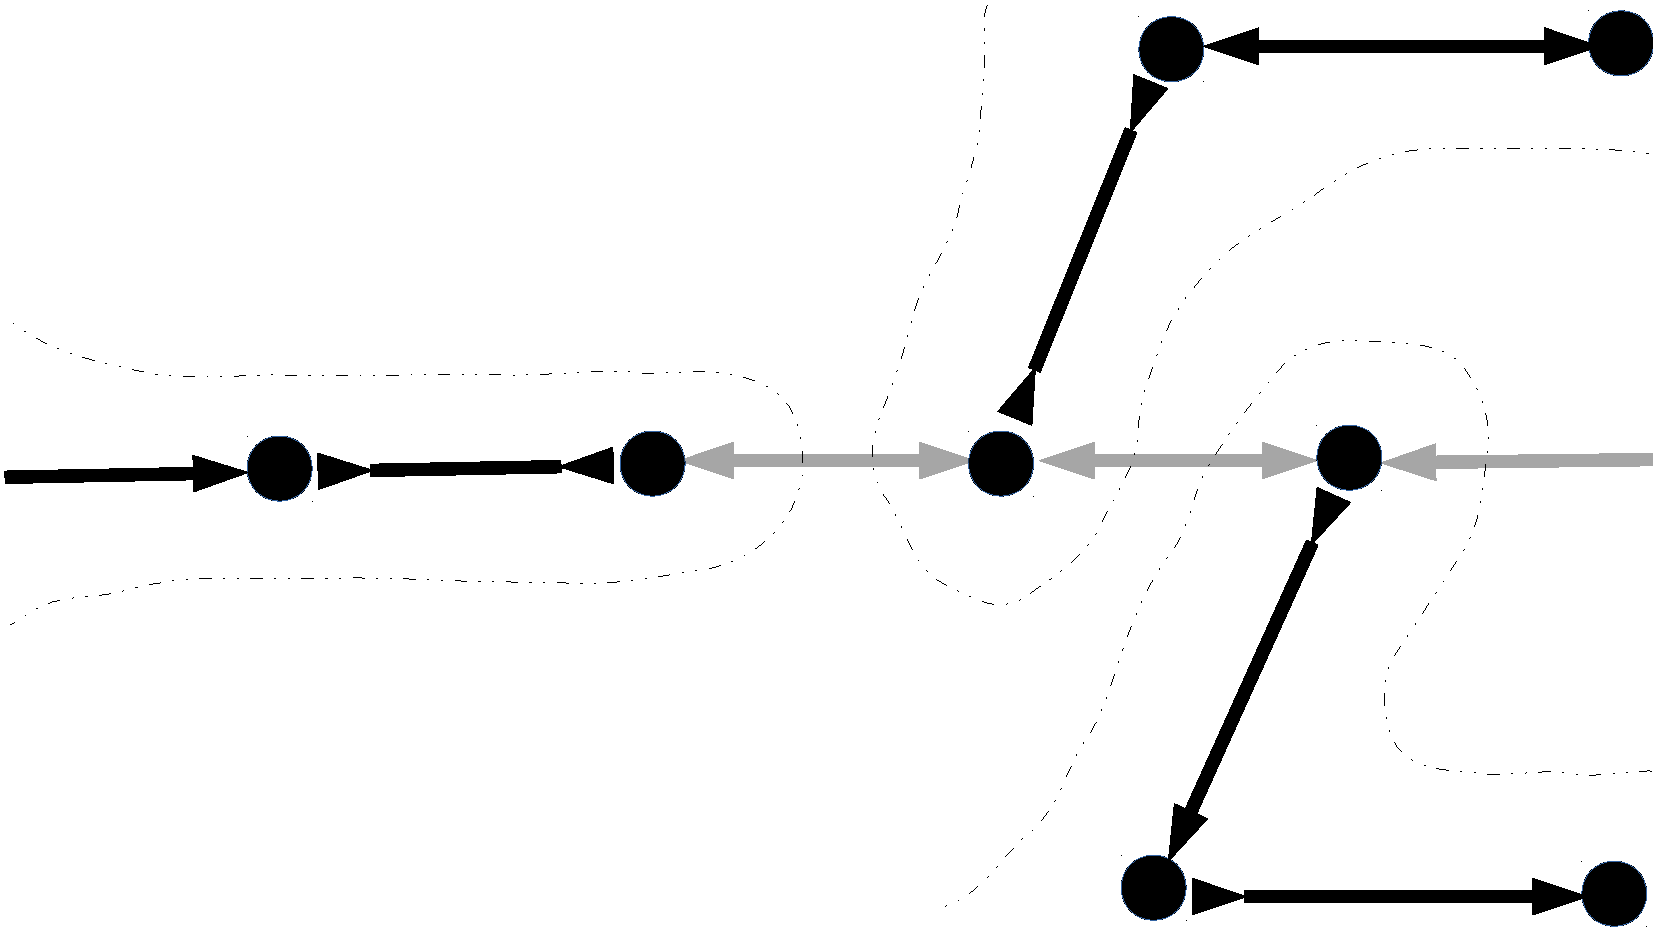
\includegraphics[width=.6\textwidth]{images/decompose.pdf}
\caption[Example of graph decomposition into longest straight paths]{Example of graph decomposition into longest straight paths. Branching edges are masked out (shaded) leaving only straight paths (bold colored) to report. There would be 3 contigs extracted by traversing along the straight paths here.}
\label{figure:npgraph_decompose}
\end{figure}
The decomposed graph is only used to report the contigs that can be extracted from an assembly graph at certain time point. For that reason, the branching edges are only masked but not removed from the original graph as they would be used for further bridging.

The final assembly output contains files in both FASTA and GFA v1 format (\url{https://github.com/GFA-spec/GFA-spec}). While the former only retains the actual genome sequences from the final decomposed graph, the latter output file can store almost every properties of the ultimate un-masked graph such as nodes, links and potential paths between them.


\bibliographystyle{pnas2011}
\bibliography{library} 

\end{document}
